\chapter{Functional Programming and Closures \label{chapter:closures}}
We have already mentioned that \setlx\ is a full-fledged functional language:
Functions can be used both as arguments to other functions and as return values.  There is
no fundamental difference between the type of a function and, say, the type of a rational
number, as both can be assigned to variables, converted to strings, used as arguments of other
functions, or returned from a function.  

Additionaly, \setlx\ supports
\href{http://en.wikipedia.org/wiki/Closure_(computer_science)}{\emph{closures}}
in a way similar to languages like \textsl{Scheme} \cite{sussman:75}. 
In order to introduce closures, we will first present some simple examples.  After that, we show
a more complex case study: We discuss a program that transforms a regular expression into a
non-deterministic finite state machine.

\section{Introductory Examples}
In this section we will first introduce the basic ideas of functional programming.
After that, we discuss the notion of a closure.

Using functions as arguments to other functions is something that is not often seen in
conventional programming languages.  Figure \ref{fig:reduce.stlx} on page \pageref{fig:reduce.stlx}
shows the implementation of the function \texttt{reduce} that takes two arguments:
\begin{enumerate}
\item The first argument is a list $l$.
\item The second argument is a binary function $f$ combining two elements of $l$ into a single value.
\end{enumerate}

\begin{figure}[!ht]
\centering
\begin{Verbatim}[ frame         = lines, 
                  framesep      = 0.3cm, 
                  firstnumber   = 1,
                  labelposition = bottomline,
                  numbers       = left,
                  numbersep     = -0.2cm,
                  xleftmargin   = 0.8cm,
                  xrightmargin  = 0.8cm,
                ]
    reduce := procedure(l, f) {
        match (l) {
            case []     : return;
            case [x]    : return x;
            case [x,y|r]: return reduce([f(x,y) | r], f);
        }    
    };
    add      := procedure(a, b) { return a + b; };
    multiply := procedure(a, b) { return a * b; };
    
    l := [1 .. 36];
    x := reduce(l, add     );
    y := reduce(l, multiply);
\end{Verbatim}
\vspace*{-0.3cm}
\caption{Implementing a second order function.}
\label{fig:reduce.stlx}
\end{figure}
The function \texttt{reduce} combines successive arguments of the list $l$ using the function $f$
and thereby reduces the list $l$ into a single value.  For example, if the function $f$ is the
function \texttt{add} that just adds its arguments, then $\texttt{reduce}(l,
\texttt{add})$ computes the sum of
the elements of $l$.  Therefore, in line 12 the invocation of
\texttt{reduce(l, add)} computes the sum
\\[0.2cm]
\hspace*{1.3cm}
 $\sum\limits_{i=1}^n i$. 
\\[0.2cm] 
Note that the expression ``\texttt{+/ $l$}'' is another way to compute this sum.
If instead the second arguments of the function \texttt{reduce} is the function
\texttt{multiply} that returns the product of its arguments, then 
$\texttt{reduce}(l, \texttt{multiply})$ computes the product of all elements of the list
$l$ and hence is equivalent to the expression ``\texttt{*/ $l$}''.
Finally, it should be noted that in the case that the list $l$ is empty,
\texttt{reduce} returns the value \texttt{om}. 


\begin{figure}[!ht]
\centering
\begin{Verbatim}[ frame         = lines, 
                  framesep      = 0.3cm, 
                  firstnumber   = 1,
                  labelposition = bottomline,
                  numbers       = left,
                  numbersep     = -0.2cm,
                  xleftmargin   = 0.8cm,
                  xrightmargin  = 0.8cm,
                ]
    sort := procedure(l, cmp) {
        if (#l < 2) { return l; }
        m := #l \ 2;
        [l1, l2] := [l[.. m], l[m+1 ..]];
        [s1, s2] := [sort(l1, cmp), sort(l2, cmp)];
        return merge(s1, s2, cmp);
    };
    merge := procedure(l1, l2, cmp) {
        match ([l1, l2]) {
            case [[], _] : return l2;
            case [_, []] : return l1;
            case [[x1|r1], [x2|r2]] : 
                 if (cmp(x1, x2)) {
                     return [x1 | merge(r1, l2, cmp)];
                 } else {
                     return [x2 | merge(l1, r2, cmp)];
                 }
        }
    };
    less    := procedure(x, y) { return x < y; };
    greater := procedure(x, y) { return y < x; };
    l  := [1,3,5,4,2];    
    s1 := sort(l, less   );
    s2 := sort(l, greater);
\end{Verbatim}
\vspace*{-0.3cm}
\caption{A generic sort function.}
\label{fig:merge-sort.stlx}
\end{figure}

Notice that the function \texttt{reduce} is a so called \emph{second order function} because
one of its arguments is itself a function.  While the example given above might seem
artificial, there are common applications of this scheme.  One example is sorting.
Figure \ref{fig:merge-sort.stlx} on page \pageref{fig:merge-sort.stlx} shows a generic
implementation of the algorithm \href{https://en.wikipedia.org/wiki/Merge_sort}{\emph{merge sort}}.
Here, the function \texttt{sort} takes two arguments:
\begin{enumerate}
\item The first argument $l$ is the list to be sorted.
\item The second argument \texttt{cmp} is a binary function that compares two  elements
      and returns either \texttt{true} or \texttt{false}.  If we call the function
      \texttt{sort} with second argument \texttt{less}, where the function \texttt{less} is
      defined in line 20, then the resulting list will be sorted ascendingly.
      If instead we use the function \texttt{greater} defined in line 21 as the second
      argument, then the list $l$ will be sorted descendingly.

      The second argument \texttt{cmp} of the procedure \texttt{sort} enables us to sort a list that
      contains elements that are not numbers.  In order to do so, we just have to implement an
      appropriate version of the function \texttt{cmp}.
\end{enumerate}
So far, the functions we have discussed did not return functions.  The next example will change
that.  In mathematics, given a function
\\[0.2cm]
\hspace*{1.3cm}
$f: \mathbb{N} \rightarrow \mathbb{N}$
\\[0.2cm]
mapping natural numbers into natural numbers, the \emph{discrete derivative} of $f$ is again a
function mapping natural numbers to natural numbers and is denoted
as $\Delta f$.  For $n \in \mathbb{N}$, the value $(\Delta f)(n)$ is defined as
\\[0.2cm]
\hspace*{1.3cm}
$(\Delta f)(n) := f(n+1) - f(n)$.
\\[0.2cm]
For example, given the function $f: \mathbb{N} \rightarrow \mathbb{N}$ defined as $f(n) := 2^n$,
we have
\\[0.2cm]
\hspace*{1.3cm}
$(\Delta f)(n) = 2^{n+1} - 2^n = 2^n = f(n)$.
\\[0.2cm]
To give another example, the discrete derivative of the identity function is the function that
maps every natural number to the number $1$, since $(n+1) - n = 1$.  

\begin{figure}[!ht]
\centering
\begin{Verbatim}[ frame         = lines, 
                  framesep      = 0.3cm, 
                  firstnumber   = 1,
                  labelposition = bottomline,
                  numbers       = left,
                  numbersep     = -0.2cm,
                  xleftmargin   = 0.8cm,
                  xrightmargin  = 0.8cm,
                ]
    delta := procedure(f) {
        return n |-> f(n+1) - f(n);
    };    
    g := n |-> n;
    h := n |-> 2 ** n;
    deltaG := delta(g);
    deltaH := delta(h);
    
    print([ deltaG(n) : n in [1 .. 10]]);
    print([ deltaH(n) : n in [1 .. 10]]);
\end{Verbatim}
\vspace*{-0.3cm}
\caption{Computing the discrete derivative of a given function.}
\label{fig:finite-difference.stlx}
\end{figure}

\noindent
Figure \ref{fig:finite-difference.stlx} shows the implementation of the function \texttt{delta}
that takes a function $f$ as input and then returns the discrete derivative of $f$.  In line 6
and 7, this function is applied to the identity function and to the function $n \mapsto 2^n$,
respectively.  The resulting functions \texttt{deltaG} and \texttt{deltaH} are then applied to
the sequence of natural numbers from 1 to 10.  In the first case, the result is a list
containing the number one ten times, while in the second case the the result is a list of the
first ten powers of two.


\subsection{Implementing Counters via Closures}
The concept of a closure is non-trivial, therefore we introduce the idea using some simple
examples.  Figure \ref{fig:counter-closure.stlx} shows the function
\texttt{createCounter}.  This function initializes the variable \texttt{count} to a given
value and then returns a procedure that increments this value.  Note that is procedure is not
defined via the keyword \texttt{procedure} but rather via the keyword \texttt{closure}.  The reason
is that this function needs access to the variable \texttt{count} that is defined outside of the
closure \texttt{counter}.  By defining the function \texttt{counter} as a \texttt{closure} rather
than a \texttt{procedure},  the function \texttt{counter} has access to th variable \texttt{count}:
It can both read its value and can even change the value.  When the function \texttt{counter} is
defined, the variable \texttt{count} is safely tucked away together with the function
\texttt{counter}.  Therefore, although the variable \texttt{count} goes out of scope once the
function \texttt{createCounter} terminates, the function \texttt{counter} still has access
to a 
copy of this variable.  Therefore, when we call the function \texttt{createCounter} in line 9, 
the variable \texttt{ctr0} is assigned a version of the function counter where the variable
\texttt{count} initially has the value 0.  Later, when we call the function \texttt{ctr0},
in line 12, this counter is incremented 3 times.  Therefore, after line 12 is executed,
the variables \texttt{u}, \texttt{v}, and \texttt{w} have the values $1$, $2$, and $3$,
respectively. 


\begin{figure}[!ht]
\centering
\begin{Verbatim}[ frame         = lines, 
                  framesep      = 0.3cm, 
                  firstnumber   = 1,
                  labelposition = bottomline,
                  numbers       = left,
                  numbersep     = -0.2cm,
                  xleftmargin   = 0.8cm,
                  xrightmargin  = 0.8cm,
                ]
    createCounter := procedure(i) {
        count   := i;
        counter := closure() {
                       count += 1;
                       return count;
                   };
        return counter;
    };   
    ctr0 := createCounter(0);
    ctr9 := createCounter(9);
    
    u := ctr0(); v := ctr0(); w := ctr0();
    x := ctr9(); y := ctr9(); z := ctr9();
\end{Verbatim}
\vspace*{-0.3cm}
\caption{Creating a counter as a closure.}
\label{fig:counter-closure.stlx}
\end{figure}

Notice that the variable \texttt{count} is defined outside the procedure
\texttt{counter}.  Still, it is accessible in the closure \texttt{counter} because \texttt{counter}
has been defined using the keyword \texttt{closure} instead of the keyword \texttt{procedure}.

You should also notice that the function \texttt{ctr9} created in line 10 gets its
\underline{own} copy of the variable \texttt{count}.  In the case of the function
\texttt{ctr9}, this copy of \texttt{count} is initialized with the value 9.  Therefore, after
we have called the function \texttt{ctr9} in line 13, the variables \texttt{x}, \texttt{y}, and
\texttt{z} will have the values $10$, $11$, and $12$. 

\subsection{Lambda Definitions for Closures}
There is a short-hand notation for the definition of a closure that can be used if the closure only
contains a single \texttt{return} statement. This short-hand notation relates to closures as lambda definitions relate to
procedures.  This short-hand notation is called a \emph{lambda closure}.  Here is a simple example:
The following two lines define a function \texttt{f} that computes the cube of its argument.
\\[0.2cm]
\hspace*{1.3cm} \texttt{c := 3;}            \\
\hspace*{1.3cm} \texttt{f := x |=> x * c;}
\\[0.2cm]
These two lines are equivalent to the following two lines:
\\[0.2cm]
\hspace*{1.3cm} \texttt{c := 3;}            \\
\hspace*{1.3cm} \texttt{f := closure(x) \{ return x * c; \};}
\\[0.2cm]
In general, the expression
\\[0.2cm]
\hspace*{1.3cm}
\texttt{x |=> \textsl{expr}}
\\[0.2cm]
is equivalent to the following expression:
\\[0.2cm]
\hspace*{1.3cm}
\texttt{closure(x) \{ return \textsl{expr}; \}}
\\[0.2cm]
If there is more than one argument to a closure, the arguments have to be enclosed in square
brackets.  For example, 
\\[0.2cm]
\hspace*{1.3cm}
\texttt{f := [x,y] |=> sqrt(x ** c + y ** c);}
\\[0.2cm]
is equivalent to
\\[0.2cm]
\hspace*{1.3cm}
\texttt{f := closure(x,y) \{ return sqrt(x ** c + y ** c); \};}

\section[Closures in Action]{Closures in Action: Generating Finite State Machines from Regular Expressions}
In this section we demonstrate a non-trivial application of closures.  We present a program that
takes a regular expression $r$ as input and  converts this regular expression into a
\href{http://en.wikipedia.org/wiki/Nondeterministic_finite_automaton}{\emph{non-deterministic finite state machine}} 
using the 
\href{http://en.wikipedia.org/wiki/Thompson's_construction_algorithm}{\emph{Thompson construction}}
\cite{hopcroft:06}.  For the purpose of this section, \emph{regular expressions} are defined inductively as
follows.
\begin{enumerate}
\item Every character $c$ is a regular expression matching exactly this character and
      nothing else.
\item If $r_1$ and $r_2$ are regular expressions,  then $r_1 \cdot r_2$ is a regular
      expression.  If $r_1$ matches the string $s_1$ and $r_2$ matches the string $s_2$,
      then $r_1 \cdot r_2$ matches the string $s_1s_2$, where $s_1s_2$ is understood as
      the concatenation of $s_1$ and $s_2$.
\item If $r_1$ and $r_2$ are regular expressions,  then $r_1 \mid r_2$ is a regular
      expression.  The regular expression $r_1 \mid r_2$ matches any string that is matched
      by either $r_1$ or $r_2$.
\item If $r$ is a regular expression, then $r^*$ is a regular expression.
      This regular expression matches the empty string and, furthermore, matches any string
      $s$ that can be decomposed as
      \\[0.2cm]
      \hspace*{1.3cm}
      $s = t_1 t_2 \cdots t_n$
      \\[0.2cm]
      where each of the substrings $t_i$ is matched by the regular expression $r$.
\end{enumerate}
For the purpose of the program we are going to develop, composite regular expressions will be
represented by terms.  In detail, we have the following representation of regular
expressions.
\begin{enumerate}
\item A regular expression $r$ of the form $r = c$ where $c$ is a single character is
      represented by the string consisting of the character $c$.
\item A regular expression $r$ of the form $r = r_1 \cdot r_2$ is represented by the term
      \\[0.2cm]
      \hspace*{1.3cm}
      \texttt{Cat(r1, r2)}
      \\[0.2cm]
      where \texttt{r1} is the representation of $r_1$ and \texttt{r2} is the
      representation of $r_2$.  The name \texttt{Cat} reminds us of con\underline{cat}enation. 
\item A regular expression $r$ of the form $r = r_1 \mid r_2$ is represented by the term
      \\[0.2cm]
      \hspace*{1.3cm}
      \texttt{Or(r1, r2)}
      \\[0.2cm]
      where \texttt{r1} is the representation of $r_1$ and \texttt{r2} is the
      representation of $r_2$.
\item A regular expression $r$ of the form $r = r_0^*$ is represented by the term
      \\[0.2cm]
      \hspace*{1.3cm}
      \texttt{Star(r0)}
      \\[0.2cm]
      where \texttt{r0} is the representation of $r_0$. 
\end{enumerate}
The \href{https://en.wikipedia.org/wiki/Thompson%27s_construction_algorithm}{\emph{Thompson construction}}
of a non-deterministic finite state machine from a given regular 
expression $r$ works by induction on the structure of $r$.  Given a regular expression
$r$,  we define a non-deterministic finite state machine $A(r)$ by induction on $r$.
For the purpose of this section, a finite state machine $A$ is a 4-tuple
\\[0.2cm]
\hspace*{1.3cm}
$A = \langle Q, \delta, q_0, q_f \rangle$
\\[0.2cm]
where $Q$ is the set of states, 
$\delta$ is the transition function and maps a pair $\langle q, c \rangle$ where $q$ is a
state and $c$ is a character to a set of new states.  If we denote the set of characters
as $\Sigma$, then the function $\delta$ has the signature
\\[0.2cm]
\hspace*{1.3cm}
$\delta: Q \times \Sigma \rightarrow 2^Q$.
\\[0.2cm]
The understanding  of $\delta(q,c)$ is that if the finite state machine $A$ is in the
state $q$ and reads the character $c$, then it can switch to any of the states in
$\delta(q,c)$.
Finally, $q_0$ is the start state and $q_f$ is the accepting state.  In the following, we
abbreviate the notion of a  
\emph{finite state machine} as fsm.
\begin{enumerate}
\item For a letter $c$ the fsm $A(c)$ is defined as
      \\[0.2cm]
      \hspace*{1.3cm}
      $A(c) = \langle \{ q_0, q_1 \}, 
                      \{ \langle q_0, c \rangle \mapsto q_1\}, q_0, q_1  \rangle$.
      \\[0.2cm]
      The set of states is given as $\{ q_0, q_1 \}$, on reading the character $c$ the
      transition function maps the state $q_0$ to $q_1$, the start state is $q_0$ and the
      accepting state is $q_1$.  This fsm is shown in Figure
      \ref{fig:aChar.eps}.  The start state $q_0$ is marked by an incoming arrow, while the
      accepting state $q_1$ is marked by a doubled boundary. 

      \begin{figure}[!ht]
        \centering
      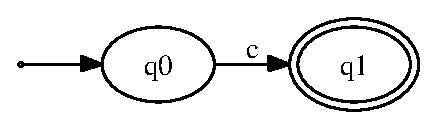
\epsfig{file=aChar.eps, scale=0.5}
      \caption{The finite state machine $A(c)$.}
      \label{fig:aChar.eps}
      \end{figure}

      \begin{figure}[!ht]
      \centering
      \begin{Verbatim}[ frame         = lines, 
                        framesep      = 0.3cm, 
                        firstnumber   = 1,
                        labelposition = bottomline,
                        numbers       = left,
                        numbersep     = -0.2cm,
                        xleftmargin   = 0.8cm,
                        xrightmargin  = 0.8cm,
                      ]
    genCharNFA := procedure(c, rw ctr) {
        q0 := getNewState(ctr);
        q1 := getNewState(ctr);
        delta := closure(q, d) { 
                     if (q == q0 && d == c) { 
                         return { q1 };
                     } else { 
                         return {};
                     }
                 };
        return [ {q0, q1}, delta, q0, q1 ];
    };
      \end{Verbatim}
      \vspace*{-0.3cm}
      \caption{Generating the fsm to recognize the character $c$.}
      \label{fig:genCharNFA.stlx}
      \end{figure}

      Figure \ref{fig:genCharNFA.stlx} shows the function \texttt{genCharNFA} that takes a
      character $c$ and generates the fsm $A(c)$.  The code corresponds to the
      diagram shown in Figure \ref{fig:aChar.eps}.
      \begin{enumerate}
      \item We generate two new states $q_0$ and $q_1$ using the function
            \texttt{getNewState}.  The implementation of this function is shown in Figure
            \ref{fig:getNewState.stlx} on page \pageref{fig:getNewState.stlx}.  It creates a new 
            unique string that is interpreted as a state.
      \item The transition function checks whether the state $q$ given as input is equal
            to the start state $q_0$ and whether, furthermore, the character $d$ that is
            read is identical to the character $c$.  If this is the case, the fsm switches
            into the state $q_1$ and therefore the set of possible next states is the singleton
            set $\{ q_1 \}$.  Since this is the only transition of the fsm, in all other
            cases the set of next states is empty.
      \end{enumerate}
      
\item In order to compute the fsm $A(r_1 \cdot r_2)$ 
      we have to assume that the sets of states of the fsms
      $A(r_1)$ and $A(r_2)$ are disjoint.  This is true since the function \texttt{getNewState} does
      create a new state every time it is called.
      Let us assume that the fsms  $A(r_1)$ and $A(r_2)$ have the following form:
      \begin{enumerate}
      \item $A(r_1) = \langle Q_1, \delta_1, q_1, q_2 \rangle$,
      \item $A(r_2) = \langle Q_2, \delta_2, q_3, q_4 \rangle$, \quad where
      \item $Q_1 \cap Q_2 = \{\}$.
      \end{enumerate}
      Using $A(r_1)$ and $A(r_2)$ we construct the fsm $A(r_1 \cdot r_2)$ as
      \\[0.2cm]
      \hspace*{0.8cm}
       $\langle Q_1 \cup Q_2, \Sigma, 
                \{ \pair(q_2,\varepsilon) \mapsto q_3 \} 
                   \cup \delta_1 \cup \delta_2, q_0, q_4 \rangle$
      \\[0.2cm]
      The notation $\{ \pair(q_2,\varepsilon) \mapsto q_3 \} \cup \delta_1 \cup \delta_2$
      specifies that the transition function $\delta$ contains all the transitions
      from the transition functions  $\delta_1$ and $\delta_2$.  Additionally,
      there is an  $\varepsilon$-transition from $q_2$ to
      $q_3$.  Formally, the transition function could also be specified as follows:
      \\[0.2cm]
      \hspace*{1.3cm}
      $\delta(q,c) := \left\{
      \begin{array}{ll}
        \{ q_3 \}       & \mbox{if $q = q_2$ and $c = \varepsilon$}, \\[0.2cm]
        \delta_1(q, c)  & \mbox{if $q \in Q_1$ and $\pair(q,c) \not= \pair(q_2,\varepsilon)$}, \\[0.2cm]
        \delta_2(q, c)  & \mbox{if $q \in Q_2$.} 
      \end{array}\right.
      $
      \\[0.2cm]
      Figure \ref{fig:aConcat.eps} depicts the fsm $A(r_1 \cdot r_2)$.
      
      \begin{figure}[!ht]
        \centering
      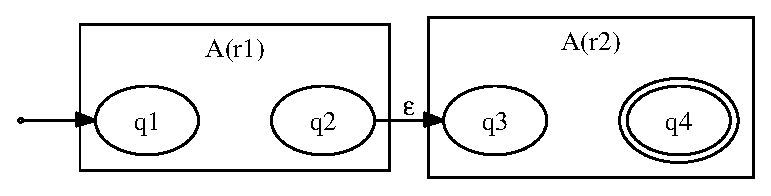
\epsfig{file=aConcat.eps, scale=0.8}
      \caption{The finite state machine $A(r_1 \cdot r_2)$.}
      \label{fig:aConcat.eps}
      \end{figure}

      Figure \ref{fig:catenate.stlx} on page \pageref{fig:catenate.stlx} shows the
      implementation of the function \texttt{catenate}.  This function takes two
      finite state machines \texttt{f1} and \texttt{f2} and concatenates them in the way
      depicted in Figure \ref{fig:aConcat.eps}.  This function can be used
      to compute $A(r_1 \cdot r_2)$, since we have
      \\[0.2cm]
      \hspace*{1.3cm}
      $A(r_1 \cdot r_2) = \mathtt{catenate}\bigl(A(r_1), A(r_2)\bigr)$.

    \begin{figure}[!ht]
    \centering
    \begin{Verbatim}[ frame         = lines, 
                      framesep      = 0.3cm, 
                      firstnumber   = 1,
                      labelposition = bottomline,
                      numbers       = left,
                      numbersep     = -0.2cm,
                      xleftmargin   = 0.8cm,
                      xrightmargin  = 0.8cm,
                    ]
    catenate := procedure(f1, f2) {
        [m1, delta1, q1, q2] := f1;
        [m2, delta2, q3, q4] := f2;
        delta := closure(q, c) {
                     if (q == q2 && c == "") {
                         return { q3 };
                     } else if (q in m1) {
                         return delta1(q, c);
                     } else if (q in m2) {
                         return delta2(q, c);
                     } else {
                         return {};
                     }
                 };
        return [ m1 + m2, delta, q1, q4 ];
    };
    \end{Verbatim}
    \vspace*{-0.3cm}
    \caption{The function to compute $A(r_1 \cdot r_2)$}
    \label{fig:catenate.stlx}
    \end{figure}
\item In order to define the fsm  $A(r_1 + r_2)$ we assume that we have already computed
      the fsms $A(r_1)$ and $A(r_2)$ and that their sets of states are disjoint.
      If  $A(r_1)$ and $A(r_2)$ are given as
      \\[0.2cm]
      \hspace*{1.3cm}
      $A(r_1) = \langle Q_1, \delta_1, q_1, q_3 \rangle$ \quad and \quad
      $A(r_2) = \langle Q_2, \delta_2, q_2, q_4 \rangle$
      \\[0.2cm]
      then the fsm $A(r_1 + r_2)$ can be defined as
      \\[0.2cm]
      \hspace*{0.0cm}
       $\langle \{ q_0, q_5 \} \cup Q_1 \cup Q_2, 
                \{ \pair(q_0,\varepsilon) \mapsto q_1, \pair(q_0,\varepsilon) \mapsto q_2,
                   \pair(q_3,\varepsilon) \mapsto q_5, \pair(q_4,\varepsilon) \mapsto q_5 \} 
                   \cup \delta_1 \cup \delta_2, q_0, q_5 \rangle$.
      \\[0.2cm]
      This finite state machine is shown in Figure \ref{fig:aPlus.eps}.
      In addition to the states of $A(r_1)$ and $A(r_2)$ there are two additional 
      states:
      \begin{enumerate}
      \item $q_0$ is the start state of the fsm $A(r_1 + r_2)$,
      \item $q_5$ is the accepting state of $A(r_1 + r_2)$.
      \end{enumerate}
      In addition to the transitions of the fsms  $A(r_1)$ and $A(r_2)$ we have four $\varepsilon$-transitions.
      \begin{enumerate}
      \item There are $\varepsilon$-transitions from $q_0$ to the states $q_1$ and $q_2$.
      \item There are $\varepsilon$-transitions from  $q_3$ and $q_4$ to $q_5$.
      \end{enumerate}
                   
      \begin{figure}[!ht]
        \centering
      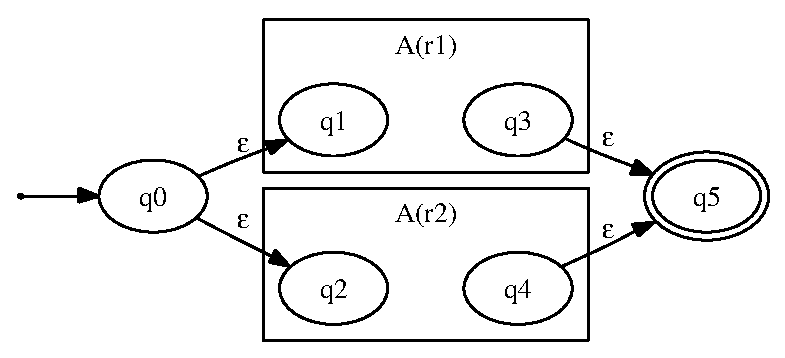
\epsfig{file=aPlus.eps, scale=0.5}
      \caption{The finite state machine $A(r_1 + r_2)$.}
      \label{fig:aPlus.eps}
      \end{figure}

    \begin{figure}[!ht]
    \centering
    \begin{Verbatim}[ frame         = lines, 
                      framesep      = 0.3cm, 
                      firstnumber   = 1,
                      labelposition = bottomline,
                      numbers       = left,
                      numbersep     = -0.2cm,
                      xleftmargin   = 0.8cm,
                      xrightmargin  = 0.8cm,
                    ]
    disjunction := procedure(f1, f2, rw ctr) {
        [m1, delta1, q1, q3] := f1;
        [m2, delta2, q2, q4] := f2;
        q0 := getNewState(ctr); 
        q5 := getNewState(ctr); 
        delta := closure(q, c) {
                     if (q == q0 && c == "") {
                         return { q1, q2 };
                     } else if (q in { q3, q4 } && c == "") {
                         return { q5 };
                     } else if (q in m1) {
                         return delta1(q, c);
                     } else if (q in m2) {
                         return delta2(q, c);
                     } else {
                         return {};
                     } 
                 };
        return [ { q0, q5 } + m1 + m2, delta, q0, q5 ];
    };
    \end{Verbatim}
    \vspace*{-0.3cm}
    \caption{The function to compute $A(r_1 + r_2)$.}
    \label{fig:disjunction.stlx}
    \end{figure}
      
      Figure \ref{fig:disjunction.stlx} on page \pageref{fig:disjunction.stlx} shows the
      implementation of the function \texttt{disjunction}.  This function takes two
      finite state machines \texttt{f1} and \texttt{f2} and combines them in the way
      depicted in Figure \ref{fig:aPlus.eps}.  This function can be used
      to compute $A(r_1 + r_2)$, since we have
      \\[0.2cm]
      \hspace*{1.3cm}
      $A(r_1 +r_2) = \mathtt{disjunction}\bigl(A(r_1), A(r_2)\bigr)$.
\item In order to define $A(r^*)$ we assume $A(r)$ is given as
      \\[0.2cm]
      \hspace*{1.3cm}
      $A(r) = \langle Q, \delta, q_1, q_2 \rangle$.
      \\[0.2cm]
      Then  $A(r^*)$ is defined as
      \\[0.2cm]
      \hspace*{0.8cm}
       $\langle \{ q_0, q_3 \} \cup Q, 
                \{ \pair(q_0,\varepsilon) \mapsto q_1, \pair(q_2,\varepsilon) \mapsto q_1,
                   \pair(q_0,\varepsilon) \mapsto q_3, \pair(q_2,\varepsilon) \mapsto q_3 \} 
                   \cup \delta, q_0, q_3  \rangle$.
      \\[0.2cm]

      \begin{figure}[!ht]
        \centering
      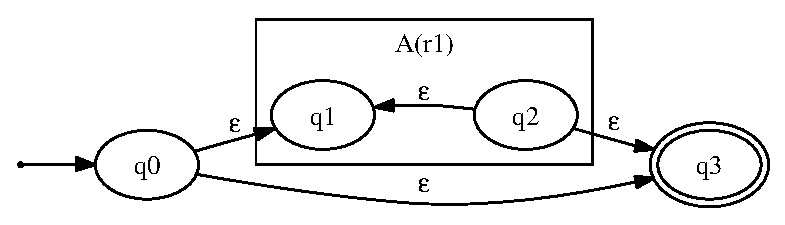
\epsfig{file=aStar.eps, scale=0.5}
      \caption{The finite state machine $A(r^*)$.}
      \label{fig:aStar.eps}
      \end{figure}

      Figure \ref{fig:aStar.eps} depicts the fsm $A(r^*)$.
      In addition to the states of the fsm  $A(r)$ there are two new states:
      \begin{enumerate}
      \item $q_0$ is the start state of $A(r^*)$,
      \item $q_3$ is the accepting state of $A(r^*)$.
      \end{enumerate}
      Furthermore, there are four additional  $\varepsilon$-transitions.
      \begin{enumerate}
      \item There are two $\varepsilon$-transitions form the start state $q_0$ to $q_1$ and $q_3$.
      \item From $q_2$ there is an  $\varepsilon$-transition back to $q_1$ and also an
            $\varepsilon$-transition to $q_3$.
      \end{enumerate}
      Figure \ref{fig:kleene.stlx} on page \pageref{fig:kleene.stlx} shows the
      implementation of the function \texttt{kleene}.  This function takes a
      finite state machine \texttt{f} and transforms it in the way
      depicted in Figure \ref{fig:aStar.eps}.  This function can be used
      to compute $A(r^*)$, since we have
      \\[0.2cm]
      \hspace*{1.3cm}
      $A(r^*) = \mathtt{kleene}\bigl(A(r)\bigr)$.
 
    \begin{figure}[!ht]
    \centering
    \begin{Verbatim}[ frame         = lines, 
                      framesep      = 0.3cm, 
                      firstnumber   = 1,
                      labelposition = bottomline,
                      numbers       = left,
                      numbersep     = -0.2cm,
                      xleftmargin   = 0.8cm,
                      xrightmargin  = 0.8cm,
                    ]
    kleene := procedure(f, rw ctr) {
        [m, delta0, q1, q2] := f;
        q0 := getNewState(ctr); 
        q3 := getNewState(ctr); 
        delta := closure(q, c) {
                     if (q == q0 && c == "") {
                         return { q1, q3 };
                     } else if (q == q2 && c == "") {
                         return { q1, q3 };
                     } else if (q in m) {
                         return delta0(q, c);
                     } else {
                         return {};
                     } 
                 };
        return [ { q0, q3 } + m, delta, q0, q3 ];
    };
    \end{Verbatim}
    \vspace*{-0.3cm}
    \caption{The function to compute $A(r^*)$.}
    \label{fig:kleene.stlx}
    \end{figure}
\end{enumerate}

Figure \ref{fig:getNewState.stlx} shows the procedure \texttt{getNewState} that is used to create
new states.  Since the parameter \texttt{ctr} of this procedure is preceded by the keyword
\texttt{rw}, this parameter has a \emph{call-by-name} semantics and therefore the procedure
\texttt{getNewState} is able to increment this variable.  Hence, the states generated
by \texttt{getNewState} are unique. 

\begin{figure}[!ht]
\centering
\begin{Verbatim}[ frame         = lines, 
                  framesep      = 0.3cm, 
                  firstnumber   = 1,
                  labelposition = bottomline,
                  numbers       = left,
                  numbersep     = -0.2cm,
                  xleftmargin   = 0.8cm,
                  xrightmargin  = 0.8cm,
                ]
    getNewState := procedure(rw ctr) {
        ctr += 1;
        return "q" + ctr;
    };
\end{Verbatim}
\vspace*{-0.3cm}
\caption{A function to generate unique states.}
\label{fig:getNewState.stlx}
\end{figure}

Finally, Figure \ref{fig:regexp2NFA.stlx} shows how to generate a finite state machine
from a given regular expression $r$.  The function $\texttt{regexp2NFA}(r)$ is defined by
recursion on $r$:
\begin{enumerate}
\item If $r$ is a single character $c$, then the fsm $A(c)$ is computed using
      the function $\texttt{genCharNFA}(c)$.
\item If $r = r_1 \cdot r_2$, the function \texttt{regexp2NFA} recursively computes
      finite state machines $A(r_1)$ and $A(r_2)$.  These fsms are then combined
      using the function $\texttt{catenate}\bigr(A(r_1), A(r_2)\bigr)$.
\item If $r = r_1 + r_2$, the function \texttt{regexp2NFA} recursively computes
      finite state machines $A(r_1)$ and $A(r_2)$.  These fsms are then combined
      using the function $\texttt{disjunction}\bigr(A(r_1), A(r_2)\bigr)$.
\item If $r = r_0^*$, the function \texttt{regexp2NFA} recursively computes
      the finite state machines $A(r_0)$.  This fsm is then transformed
      using the function $\texttt{kleene}\bigr(A(r_0)\bigr)$.
\end{enumerate}
The reader should note that we have made heavy use of closures to implement the functions
\texttt{genCharNFA}, \texttt{catenate}, \texttt{disjunction}, and \texttt{kleene}.

\begin{figure}[!ht]
\centering
\begin{Verbatim}[ frame         = lines, 
                  framesep      = 0.3cm, 
                  firstnumber   = 1,
                  labelposition = bottomline,
                  numbers       = left,
                  numbersep     = -0.2cm,
                  xleftmargin   = 0.0cm,
                  xrightmargin  = 0.0cm,
                ]
    regexp2NFA := procedure(r, rw ctr) {
        match (r) {
            case c | isString(c): 
                 return genCharNFA(c, ctr);
            case Cat(r1, r2):
                 return catenate(regexp2NFA(r1, ctr), regexp2NFA(r2, ctr)); 
            case Or(r1, r2):
                 return disjunction(regexp2NFA(r1, ctr), regexp2NFA(r2, ctr), ctr);
            case Star(r0):
                 return kleene(regexp2NFA(r0, ctr), ctr);
        }
    };
\end{Verbatim}
\vspace*{-0.3cm}
\caption{Generating a non-deterministic fsm from a regular expression.}
\label{fig:regexp2NFA.stlx}
\end{figure}

\section{Decorators}
The programming language \href{https://www.python.org}{\textsl{Python}} has a nice feature called 
\href{http://en.wikipedia.org/wiki/Python_syntax_and_semantics#Decorators}{\emph{decorators}} that
makes it easy to modify existing functions.  For example, a trace decorator is a function that can
modify a given function $f$ so that every invocation of the function $f$ and every value returned by
the function $f$ are automatically traced.  \setlx\ supports similar techniques as \textsl{Python} and,
therefore, it is easy to implement decorators in \setlx, too.  In this section, we show how a simple
albeit powerful trace decorator can be implemented in just a few lines of \setlx\ code.

\begin{figure}[!ht]
\centering
\begin{Verbatim}[ frame         = lines, 
                  framesep      = 0.3cm, 
                  firstnumber   = 1,
                  labelposition = bottomline,
                  numbers       = left,
                  numbersep     = -0.2cm,
                  xleftmargin   = 0.8cm,
                  xrightmargin  = 0.8cm,
                ]
    gcd := procedure(n, m) {
        if (m == 0) {
            return n;
        }
        return gcd(m, n % m);
    };
    myTracer := tracer();
    gcd := myTracer.trace(gcd, "gcd");
    n   := gcd(36, 27);
    gcd := myTracer.untrace("gcd");
\end{Verbatim}
\vspace*{-0.3cm}
\caption{Using the trace decorator.}
\label{fig:tarce-decorator-use.stlx}
\end{figure}

Figure \ref{fig:tarce-decorator.stlx} on page \pageref{fig:tarce-decorator.stlx} shows the class
\texttt{trace}.  This class implements a trace decorator.  Before we discuss the details of its
implementation, lets us show how this decorator is used.  Figure \ref{fig:tarce-decorator-use.stlx}
shows the implementation of the function \texttt{gcd} computing the greatest common divisor of two
natural numbers using the \href{http://en.wikipedia.org/wiki/Euclidean_algorithm}{Euclidean algorithm}.
Suppose we want to trace every invocation of the function \texttt{gcd}.  We do so by first creating
an object of class \texttt{tracer} in line 7 of Figure \ref{fig:tarce-decorator-use.stlx}.  Then the line
\\[0.2cm]
\hspace*{1.3cm}
\texttt{gcd := myTracer.trace(gcd, "gcd");}
\\[0.2cm]
activates tracing for the function \texttt{gcd}.  Note that the first argument of the method
\texttt{trace} is the function we want to trace, while the second argument is the name of the function.
After executing this assignment statement, the function \texttt{gcd} will be traced.
For example, the call \texttt{gcd(36, 27)} produces the following output:
\begin{verbatim}
    calling gcd(36, 27)
    calling gcd(27, 9)
    calling gcd(9, 0)
    gcd(9, 0) = 9
    gcd(27, 9) = 9
    gcd(36, 27) = 9
    ~< Result: 9 >~
\end{verbatim}
This shows that every time the function \texttt{gcd} is called, a statement of the form
\\[0.2cm]
\hspace*{1.3cm}
\texttt{calling gcd($m$, $n$)}
\\[0.2cm]
is printed.  This is true even for the recursive invocations of \texttt{gcd}.  Furthermore,
every time the function \texttt{gcd} returns a result, this is also printed together with the
arguments used to compute this result.

To stop tracing the function \texttt{gcd}, we simply issue the statement:
\\[0.2cm]
\hspace*{1.3cm}
\texttt{gcd := myTracer.untrace("gcd");}
\\[0.2cm]
After this assignment, the function \texttt{gcd} is restored to its original state and will not print
anything when called.

\begin{figure}[!ht]
\centering
\begin{Verbatim}[ frame         = lines, 
                  framesep      = 0.3cm, 
                  firstnumber   = 1,
                  labelposition = bottomline,
                  numbers       = left,
                  numbersep     = -0.2cm,
                  xleftmargin   = 0.8cm,
                  xrightmargin  = 0.8cm,
                ]
    class tracer() {
        mStoredProcedures := {};
        
        trace := procedure(function, functionName) {
            mStoredProcedures[functionName] := function;
            tracedFunction := closure(*args) {
                argsString := args + "";
                argsString := argsString[2..-2];
                print("calling $functionName$($argsString$)");
                result := function(*args);
                print("$functionName$($argsString$) = $result$");
                return result;
            };
            return tracedFunction;
        };
        untrace := procedure(functionName) {
            return mStoredProcedures[functionName];
        };
    }
\end{Verbatim}
\vspace*{-0.3cm}
\caption{A class providing a trace decorator.}
\label{fig:tarce-decorator.stlx}
\end{figure}

Let us proceed to discuss how the class \texttt{tracer} is implemented in \setlx.  Figure
\ref{fig:tarce-decorator.stlx} shows the implementation of this class.  We discuss this
implementation line by line.
\begin{enumerate}
\item Line 2 defines the member variable \texttt{mStoredProcedures}.  This variable will store a map
      that is represented as a binary relation.  The keys of this maps are procedure names, while the
      values entered into this map are the procedures themselves.  Initially, this map is empty.  Every time a
      procedure is traced, the old value of the procedure is stored in this map.  This is needed in
      order to implement the method \texttt{untrace} that restores a given procedure to its original
      state.
\item The workhorse of the class \texttt{tracer} is the method \texttt{trace} defined in line 4.
      This method takes two arguments:  The first argument is a procedure, while the second argument
      is the name of the procedure.  The function will return a new procedure that behaves like the
      given procedure but, furthermore, traces the invocation of the original procedure as discussed
      previously in the example.  The procedure \texttt{trace} works as follows:
      \begin{enumerate}
      \item In line 5, the old value of the procedure to be traced is saved in the dictionary 
            \\[0.2cm]
            \hspace*{1.3cm}
            \texttt{mStoredProcedures}.
      \item Next, line 6 defines a closure called \texttt{tracedFunction}.  This is a function    
            called with a variable number of arguments.  The reason is that we do
            not know how many 
            arguments the procedure \texttt{function} that is given as argument to the method
            \texttt{trace} actually takes.  In the example discussed above, we had traced the
            function \texttt{gcd} that takes two arguments.  We could just as well have traced a
            procedure taking only one argument as we could have traced a procedure taking nine
            arguments.
      \item In line 7 to 9, the closure \texttt{tracedFunction} constructs a string containing the
            arguments and the name of the function and then prints this string.  This
            \texttt{tracedFunction} refers to \texttt{function} and \texttt{functionName}.  As these
            variables  are only defined in the method \texttt{trace}, the function \texttt{tracedFunction} needs to
            be defined as a closure so that it can access these variables.
      \item Line 10 is the most important line of the whole implementation:  It is here that the
            original procedure is called with the given arguments.  Note how prefixing the list of
            arguments \texttt{args} with the operator ``\texttt{*}'' makes it possible to call this
            function without knowing how many arguments the procedure takes.
      \item Line 11 print the result that has been computed by the \texttt{function}.
      \item This result is returned in line 12.
      \item Finally, the method \texttt{trace} returns the newly created closure.  By assigning this
            closure to the name of the original procedure we can thus trace the procedure.
      \end{enumerate}
\item As a convenience, the class \texttt{tracer} also provides the method \texttt{untrace} in
      line 16.  This procedure looks up the original procedure stored under the given name in the
      dictionary \texttt{mStoredProcedures} and returns it.  Hence, assigning the value returned by
      this procedure to the name of a procedure stops tracing this procedure.
\end{enumerate}


%%% Local Variables: 
%%% Mode: Latex
%%% TeX-master: "tutorial"
%%% End: 
